\chapter{System design}
This chapter aims to familiarize the reader with architecture of our application. The system consists of two logical parts: \textbf{public website} and \textbf{private administration}. The private administration is secured with simple login/password, allowing access only to authorized personnel.
\par
When designing such system, an object-oriented approach and grouping of similar functions together is a must. There are \textbf{objects that have to be moved around our web application}, as described in the previous chapter. These objects will be: post, user, club, cup, position, and region. Thus, we came up with a \textbf{concept of managers}. Each page of SwimmPair is composed of the same/unified header, menu, and footer. The content part is filled with the page’s specific results of manager calls used to construct the data UI page layout. These managers are included and used in all pages via the start file.
\section{Technologies}
There are several technologies and tools used for creating the application.
\begin{itemize}
    \item \textbf{HTML} is HyperText Markup Language \footnote{\citep{HTML5Standard}} - application pages are templated by PHP.
    \item \textbf{CSS} is Cascading Style Sheets \footnote{\citep{CSS3Standard}}.
    \item \textbf{PHP} is a general-purpose scripting language geared toward web development \footnote{\citep{PHP74Standard}} - object model and backend services are delivered by PHP.
    \item \textbf{JavaScript}  is a general-purpose scripting language that conforms to the ECMAScript specification \footnote{\citep{ECMADocu}}.
    \item \textbf{MySQL} is an open-source relational database management system \footnote{\citep{MySQLDocu}}.
    \item \textbf{Git} is a distributed version control system: tracking changes in any set of files - this project is versioned and kept in project GitHub repository \footnote{\url{https://github.com/KlosStepan/SwimmPair-Www}}.
    \item \textbf{Docker} is a set of platform as a service products that use OS-level virtualization to deliver software in packages called containers \footnote{\citep{DockerDocu}} - used for deployment of our application.
    \item \textbf{GitHub Actions} is a platform for automating workflows in GitHub repositories - our application uses GitHub Actions to automate testing. Specifically, we checkout with \textbf{actions/checkout@v3} and then run PHP using \textbf{shivammathur/setup-php@v2} for our backend tests using PHPUnit, along with a \textbf{docker container of our database filled with database schema} for integration testing. After each push we can see success of CI wokload run.
    \item \textbf{Kubernetes} is an open-source container orchestration system for automating software deployment, scaling, and management \footnote{\citep{K8sDocu}} - used for production deployment of our application.
    \item \textbf{Redis} is an in-memory data store often used for caching, messaging, and session persistence. Our application uses Redis to store session data and share it between running container instances, allowing traffic to be efficiently redirected and load-balanced.
\end{itemize} 
\newpage
\section{Architecture overview}
A visitor comes to the \textbf{app page} where \textbf{managers} are included. From the page, there are API calls on managers that retrieve and store data as follows (\autoref{fig2.1:appschema}).
\newline
\begin{figure}[h]	
	\centering	
    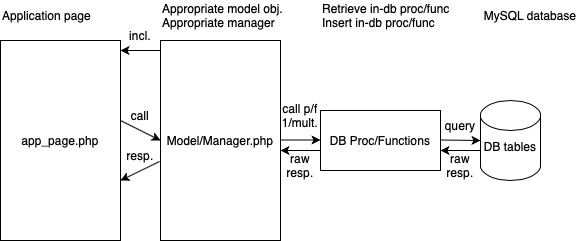
\includegraphics[scale=0.707]{img/app-schema.jpg}
	\caption{From page to manager-database function-database and back.}
	\label{fig2.1:appschema}
\end{figure}
\section{Model Managers}
Managers are designed to provide API functionality for the system administration. Managers populate pages with data and process new input from users, administering the storage of this data. Each object has a corresponding manager responsible for handling it, which helps to accommodate database loads and stores. These operations are controlled by transactions to ensure data consistency.
\newline
\textbf{Classes and their corresponding managers:}
\begin{itemize}
    \item Cup / CupsManager,
    \item User / UsersManager,
    \item Club / ClubsManager,
    \item Page / PagesManager,
    \item Post / PostsManager,
    \item Position / PositionsManager,
    \item Region / RegionsManager.
\end{itemize}
Managers are designed to retrieve and store data related to the class they are named after.
\newpage
\section{User Interface mockups}
In this chapter, we present UI mockups for both public and private parts of our application. These mockups serve as an initial visualizations of the real UI and should not be considered exact guidelines. Instead, they provide a starting point for readers and stakeholders to understand the overall direction of the UI design.
\subsection*{Public website mockups}
This part is concerned with displaying view-only data for public access.
\begin{figure}[h]	
	\centering	
    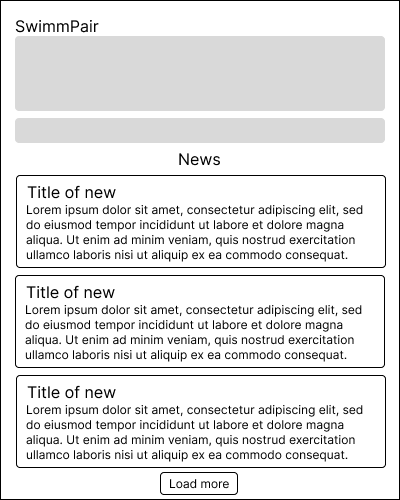
\includegraphics[scale=0.457]{img/def-U-Main.png}
    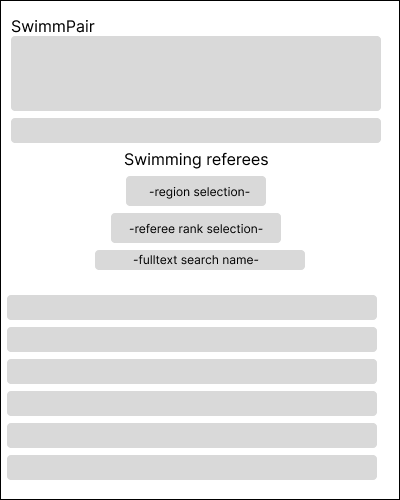
\includegraphics[scale=0.457]{img/def-U-ListingUsers.png}
    %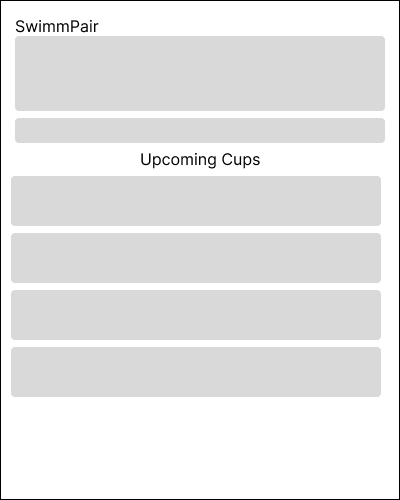
\includegraphics[scale=0.507]{img/def-U-ListingCups.png}
    %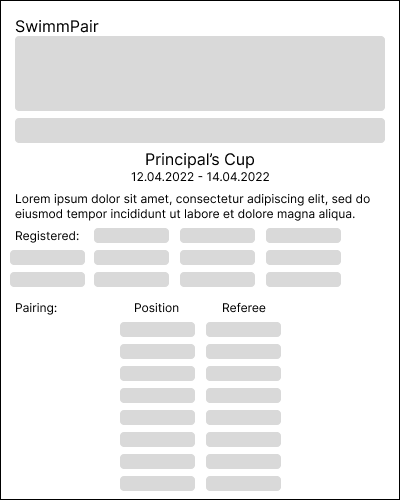
\includegraphics[scale=0.507]{img/def-U-Cup.png}
	\caption{Public pages - \underline{homepage (S5)} and \underline{listing of users (R3/S4)}.}
	\label{fig2.2:fepublicpages1}
\end{figure}
\begin{figure}[h]	
	\centering	
    %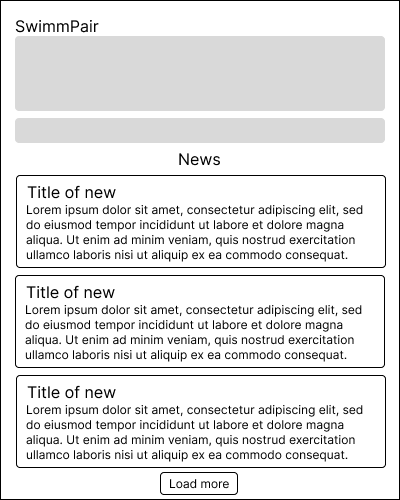
\includegraphics[scale=0.507]{img/def-U-Main.png}
    %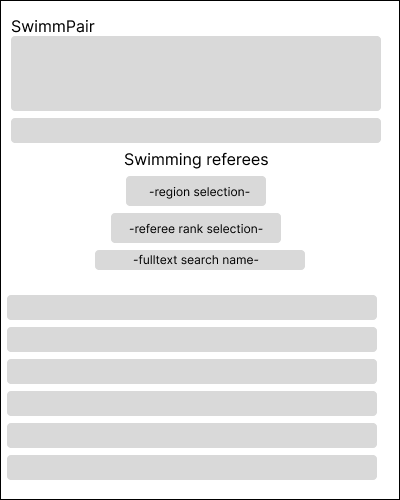
\includegraphics[scale=0.507]{img/def-U-ListingUsers.png}
    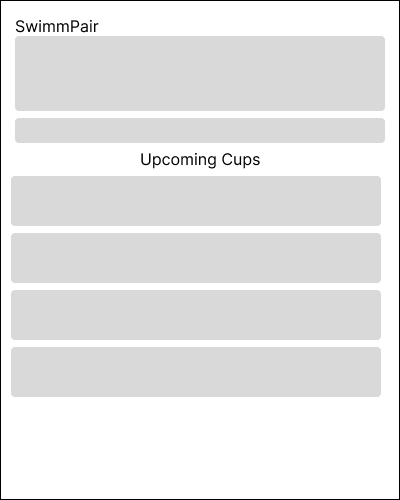
\includegraphics[scale=0.457]{img/def-U-ListingCups.png}
    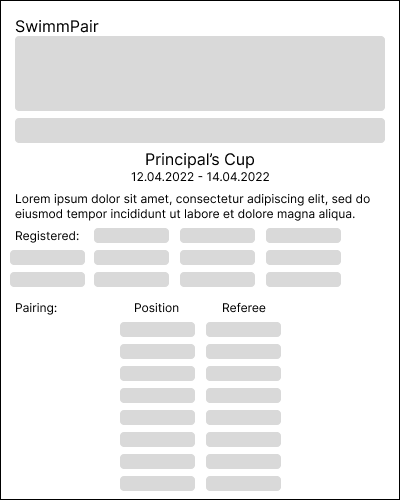
\includegraphics[scale=0.457]{img/def-U-Cup.png}
	\caption{Public pages - \underline{cups listing and cup preview (C3)}.}
	\label{fig2.3:fepublicpages2}
\end{figure}
%\newline
%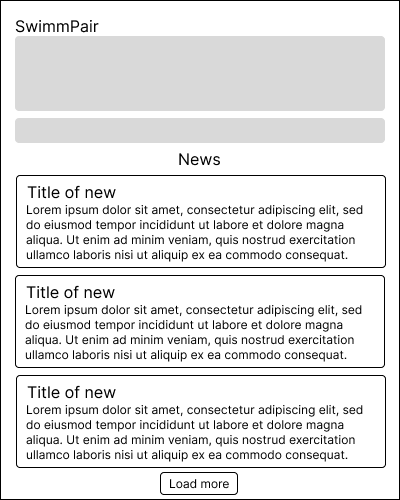
\includegraphics[scale=0.507]{img/def-U-Main.png}
%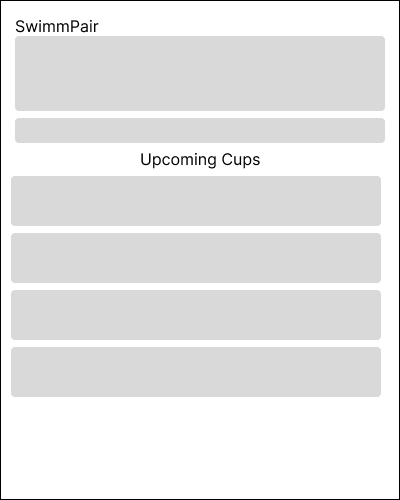
\includegraphics[scale=0.507]{img/def-U-ListingCups.png}
%\newline
%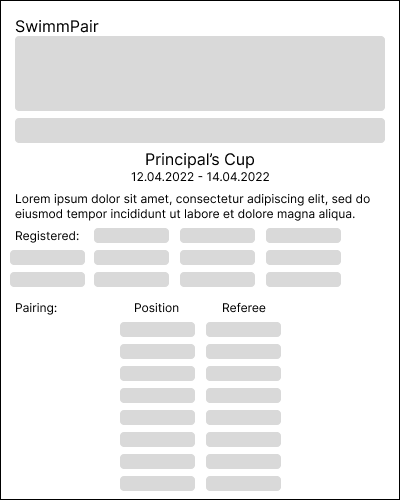
\includegraphics[scale=0.507]{img/def-U-Cup.png}
%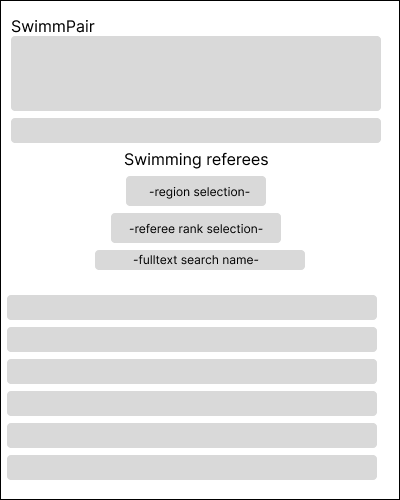
\includegraphics[scale=0.507]{img/def-U-ListingUsers.png}
\newpage
\subsection*{Administration mockups}
After logging in, the user can access the administrative menu, which is tailored to their level of access (2/1/0). This menu provides a list of administrative functions related to various aspects of the application. In the following sections, we will present mockups that demonstrate how these functional requirements may be programmed and designed.
\begin{figure}[h]	
	\centering	
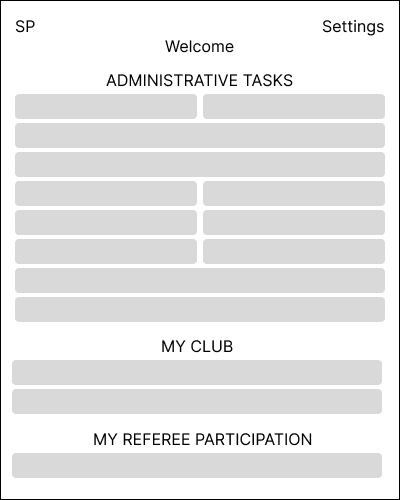
\includegraphics[scale=0.457]{img/A-administrace.png}
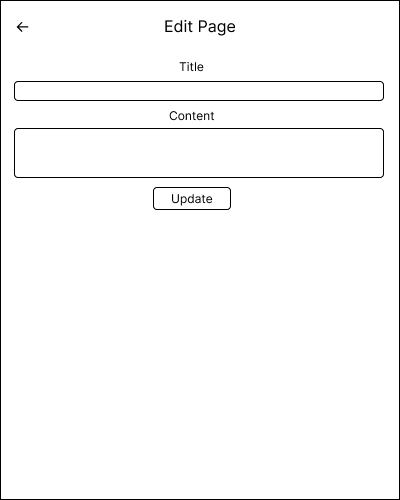
\includegraphics[scale=0.457]{img/A-edit-page.png}
\caption{Administration menu gets assembled for rights, \underline{page edit (S6)}.}
\label{fig2.4:feprivatepages1}
\end{figure}
\begin{figure}[h]	
	\centering
    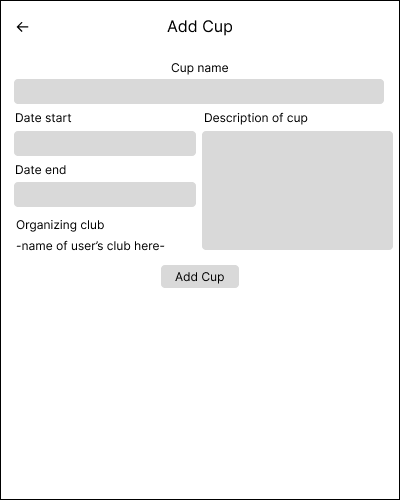
\includegraphics[scale=0.457]{img/A-new-cup.png}
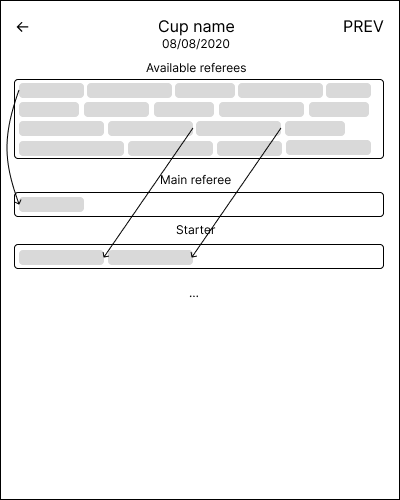
\includegraphics[scale=0.457]{img/A-pairing.png}
\caption{\underline{Add Cup (C1)} and \underline{drag'n'drop pairing (C2)}.}
\label{fig2.5:feprivatepages2}
\end{figure}
\newpage
\section{Database design}
In this chapter, we will discuss the importance of a well-defined database schema that accurately models the functional requirements and entities (\autoref{fig1.2:uml}) of the system. To achieve this, we will illustrate the process of converting real-world requirements into a rigorous database schema, highlighting the necessary mappings and merges. By doing so, we aim to design a robust system that accurately represents the needs of the stakeholders.
\subsection*{People entities merge}
We've merged three entities (\textbf{coordinator}, \textbf{club manager}, and \textbf{referee}) that model people into a single object called user, which includes additional parameters such as access rights and club affiliation to be able to distinguish  between them.
\begin{figure}[h]	
	\centering	
    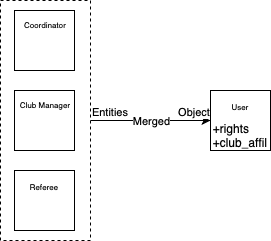
\includegraphics[scale=0.5]{img/entities_to_user.png}
	\caption{These 3 people entities got merged into one single object.}
	\label{fig2.6:enttousr}
\end{figure}
\subsection*{Pairing of entities as 3-tuple object}
Majority of logic here is modelled as entities converted to objects. Furthemore, the \textbf{availability} must preceed \textbf{pairing} in the process.
\begin{figure}[h]	
	\centering	
    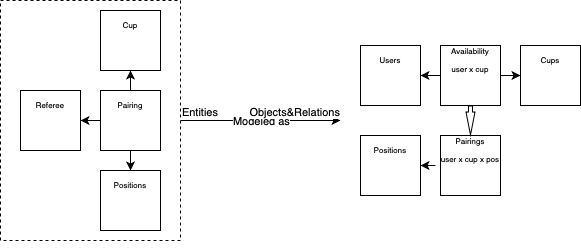
\includegraphics[scale=0.5]{img/entities_pairing_to_obj_rels.png}
	\caption{Entities modeled as 3 objects and 2 relational tables.}
	\label{fig2.7:entrels}
\end{figure}
\subsection*{Remaining entities}
The process of modeling the remaining entities as objects is relatively straightforward and self-evident. For example News from homepage are objects called Post and Regions are simply Region objects; and so on...
\newpage
\subsection*{Full database schema used for our application}
Based on all these merges, conversions and connections we can assemble a full database schema (\autoref{fig2.8:dbschemafull}) with all columns for fields in the objects.
\begin{figure}[h]	
	\centering	
    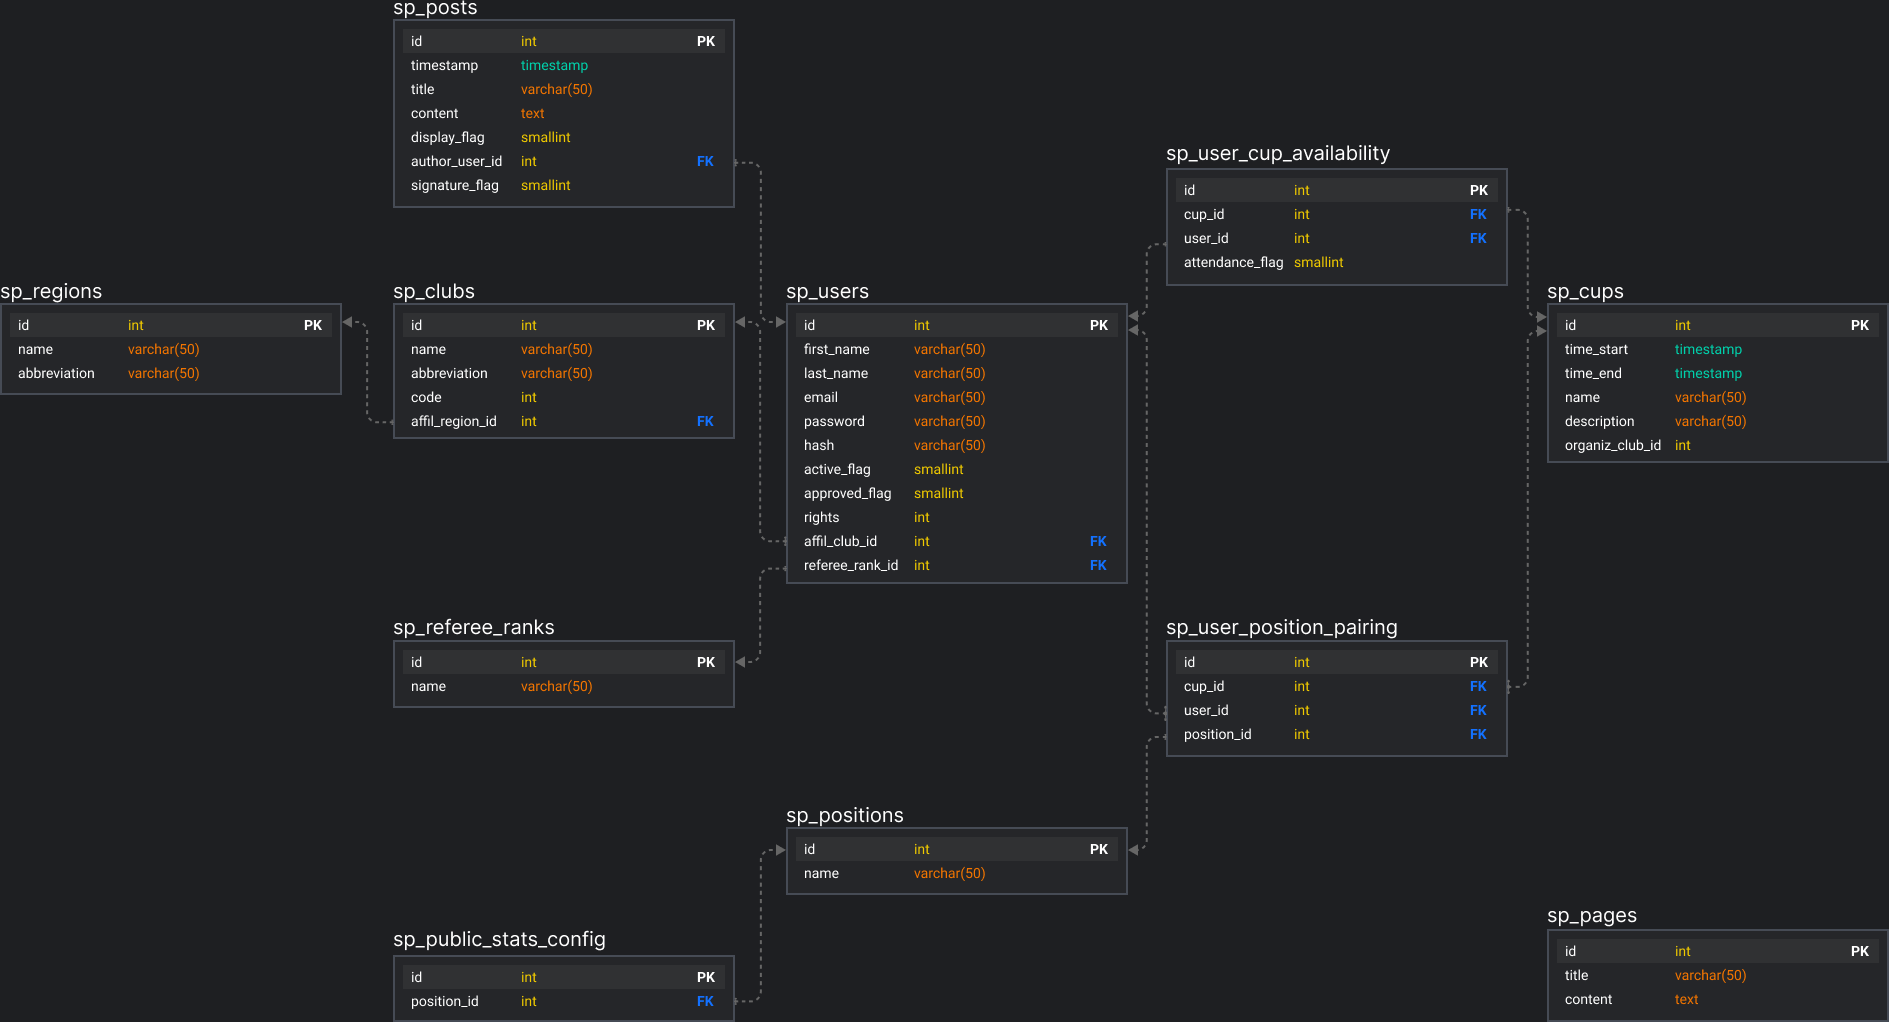
\includegraphics[scale=0.2175]{img/swimmpair_db_schema.png}
	\caption{Full database schema of our application.}
	\label{fig2.8:dbschemafull}
\end{figure}

\iffalse
% Let's take PostsManager as an example. This manager handles Post and is implemented as follows.
\textbf{Object - Post.php}
\begin{lstlisting}
class Post
{
    public $id;
    public $timestamp;
    public $title;
    public $content;
    public $display_flag;
    public $author_user_id;
	public $signature_flag;

    public function __construct($id, $timestamp, $title, $content, $display_flag, $author_user_id, $signature_flag)

	//7/7: {id, timestamp, title, content, display_flag, author_user_id, signature_flag}
	public function Serialize()
}

\end{lstlisting}
\textbf{Manager - PostsManager.php} 
\begin{lstlisting}
class PostsManager
{
	private $mysqli;

    //Constructor - setting $mysqli to $this->mysqli
	public function __construct(mysqli $mysqli)

    //Handling functions retrieve/store  
	public function GetPostById($id)
  	public function FindLastNPosts($N)
	public function InsertNewPost($title, $content, $display_flag, $author, $signature_flag)
    public function UpdatePost($id, $title, $content, $display_flag, $signature_flag)

    //Private functions - auxiliary controller functions
	private function _CreatePostOrNullFromStatement(mysqli_stmt $statement)
	private function _CreatePostsFromStatement(mysqli_stmt $statement)
	private function _CreatePostFromRow(array $row)
}
\end{lstlisting}
\textbf{Demonstration - public function GetPostById(\$id)}
\begin{lstlisting}
public function GetPostByID($id)
{
	$statement = $this->mysqli->prepare("CALL `GetPostById`(?);");
	$statement->bind_param('i', $id);
	return $this->_CreatePostOrNullFromStatement($statement);
}
\end{lstlisting}
Objects and their managers are made in the same manner. They contain different set of data and different number public functions. Description is included in documentation chapter below. 
\fi
\iffalse
\section{Responsive layout}
Listed media queries are used to provide design of the web by manually overriding specific classes for desired user experience outcome.
\begin{itemize}
    \item Basic CSS design
    \item @media (max-width: 768px)
    \item @media (print)
\end{itemize}
\textbf{Basic CSS design} gives definition of colors and desktop layout of our application. \textbf{Media query with max-width: 768px} supports tablets and mobile devices while \textbf{media print} of cup pairing hides redundant controll and informative elements while it keeps the pairing of cup to be printed.
\fi
\iffalse
\section{Administrative tasks}
\begin{itemize}
    \item \textbf{Add Post/Edit Post} - from PostsManager call \newline InsertNewPost/UpdatePost
    \item \textbf{Approve Newly Registered Users} - swap flag \textbf{approved} to \textbf{1}
    \item \textbf{Pair Available Users On Cup Positions} - from UsersManager call UpdatePairing - calls several SQL Procs for different things in transaction and commits/rollbacks
    \item \textbf{Add User/Edit User} - from UsersManager call AddUser/UpdateUser
    \item \textbf{Add Cup/Edit Cup} - from CupsManager call AddCup/UpdateCup
    \item \textbf{Add Club/Edit Club} - from ClubsManager call AddClub/UpdateClub
    \item \textbf{Add Region/Edit Region} - from RegionsManager call AddRegion/UpdateRegion
    \item \textbf{Configure Stats Ordering} - delete ordering, insert ordering \textbf{Nth}-\textbf{statId} 
    \item \textbf{Edit Contacts} - from PagesManager call UpdatePage
\end{itemize} 
\section{Club Manager tasks}
\begin{itemize}
    \item \textbf{Add Cup} - from CupsManager call AddCup
    \item \textbf{Sign Up People From My Club As Available For Cup} - prihlasit\_moje\_lidi\_na.php then XMLHttpRequest/call\_update\_availability.php
\end{itemize}   
\section{Referee tasks}    
\begin{itemize}
    \item \textbf{Sign Myself As Available For Cup} - add my Id to table \textbf{cupId}-\textbf{userId}
\end{itemize}
\fi
\newpage
\section {Functional requirements mapping to API}
We will demonstrate how specific administrative tasks, as outlined in the functional requirements, are achieved through the use of model API functions \footnote{\url{http://docu-swimmpair.stkl.cz/functions_func.html}}.
\newline
Table has following structure: \textbf{Task} - \textbf{Role} - \textbf{Function(s)}.
\newline
\begin{tabularx}{1.0\textwidth} { 
  | >{\raggedright\arraybackslash}X 
  | >{\centering\arraybackslash}X 
  | >{\raggedright\arraybackslash}X | }
 \hline
 Add Post & system admin& InsertNewPost \\
 \hline
 Edit Post  & system admin  & UpdatePost \\
 \hline
 Approve New Users & system admin & SetApprovedForUser \\
 \hline
 Create Pairing For Cup & system admin & DeleteOldPairing
InsertNewPairing\\
 \hline
 Add User & system admin & RegisterUser \\
 \hline
 Edit User & system admin &
 SetLoginEmailForUser
 SetRefereeRankForUser
 SetPasswordForUser\\
 \hline
 Add Club & system admin & InsertNewClub \\
 \hline
 Edit Club & system admin & UpdateClub \\
 \hline
 Add Region & system admin & InsertNewRegion \\
 \hline
 Edit Region & system admin & UpdateRegion \\
 \hline
 Configure Stats & system admin & DeleteOldStatsPositions
 InsertNewStatPosition \\
 \hline
 Edit Contacts & system admin & UpdatePage \\
 \hline
 Add Cup & club manager & InsertNewCup \\
 \hline
 Sign People From My Club Available For Cup & club manager & DeleteOldAvailability
 InsertNewAvailability \\
 \hline
 Sign Myself As Available For Cup & referee & SetAvailabilityRegister
 SetAvailabilityCantGo 
 SetAvailabilityCanGo \\
\hline
\end{tabularx}
\iffalse
These functions are used for \underline{retrieving} data to navigate across the administration.
\begin{itemize}
    \item Posts: FindAllPostsOrderByIDDesc
    \item Approve Users: FindAllInactiveUsersOrderByLastNameAsc
    \item Cups For Pairings: FindAllUpcomingCupsEarliestFirst
    \item Users: FindAllUsers
    \item Clubs: FindAllClubs
    \item Regions: FindAllRegions
    \item Stats: FindAllPositions, DisplayedLiveStatsConfiguredPositions
    \item Pages: GetPageByID
    \item Sign People From My Club Available For Cup : FindAllUpcomingCupsEarliestFirst, GetCupByID, FindAllTeamMembers, FindAllRegisteredTeamMembersForTheCup
    \item Sign Myself As Available For Cup: FindAllUpcomingCupsEarliestFirst, GetCupByID, IsUserAvailableForTheCup, IsComing
\end{itemize}
\fi